\documentclass{article}

\PassOptionsToPackage{numbers,sort&compress}{natbib}
\usepackage[eandd]{neurips_2026}
\usepackage[utf8]{inputenc}
\usepackage[T1]{fontenc}
\usepackage{microtype}
\usepackage{booktabs}
\usepackage{tabularx}
\usepackage{graphicx}
\usepackage{amsmath,amssymb}
\usepackage{tikz}
\usepackage{enumitem}
\usepackage{xcolor}
\usepackage{xurl}
\usepackage{seqsplit}
\usepackage{hyperref}
\usepackage[capitalise,noabbrev]{cleveref}
\usetikzlibrary{arrows.meta,positioning,fit,backgrounds}

\definecolor{FBBlue}{HTML}{1769AA}
\definecolor{FBGold}{HTML}{E6A11A}
\definecolor{FBTeal}{HTML}{168C7A}
\definecolor{FBRed}{HTML}{C75450}
\definecolor{FBCharcoal}{HTML}{262B33}
\definecolor{FBPaper}{HTML}{F7F8FA}
\hypersetup{
  colorlinks=true,
  linkcolor=FBBlue,
  citecolor=FBBlue,
  urlcolor=FBBlue,
  pdftitle={FlavourBench: An Executable Benchmark for Culinary Reasoning
    Without a Model Judge},
  pdfauthor={Anonymous Authors},
  pdfsubject={Executable culinary reasoning across frontier language models with a matched
    Epicure intervention},
  pdfkeywords={frontier language models, benchmarks, tool use, culinary reasoning,
    executable evaluation}
}
\setlist{leftmargin=*,nosep}

\newcommand{\system}{\textsc{FlavourBench}}
\newcommand{\epicure}{\textsc{Epicure}}
\newcommand{\sha}[1]{\texttt{\seqsplit{#1}}}
\newcommand{\FBReleaseSHA}{\texttt{603e4aa4db86\ldots}}
\newcommand{\FBModels}{20}
\newcommand{\FBTasks}{32}
\newcommand{\FBPairs}{640}
\newcommand{\FBArms}{1280}
\newcommand{\FBObservedArms}{1195}
\newcommand{\FBMissingArms}{85}
\newcommand{\FBTopModel}{GPT-5.6 Sol Pro}
\newcommand{\FBTopScore}{62.5}
\newcommand{\FBTopCorrect}{20}
\newcommand{\FBTopOnCorrect}{32}
\newcommand{\FBTopUplift}{+37.5}
\newcommand{\FBBottomModel}{Nemotron 3 Ultra}
\newcommand{\FBBottomScore}{0.0}
\newcommand{\FBBottomCorrect}{0}
\newcommand{\FBAggregateOff}{43.9}
\newcommand{\FBAggregateOn}{93.9}
\newcommand{\FBAggregateUplift}{+50.0}
\newcommand{\FBToolCalls}{606}
\newcommand{\FBReferenceMatches}{606}
\newcommand{\FBObservedCost}{5.19}
\newcommand{\FBPositiveUpliftModels}{19}
\newcommand{\FBNegativeUpliftModels}{0}
\newcommand{\FBZeroUpliftModels}{1}
\newcommand{\FBBestUpliftModel}{Mistral Large 2512}
\newcommand{\FBBestUplift}{+93.8}
\newcommand{\FBWorstUpliftModel}{Nemotron 3 Ultra}
\newcommand{\FBWorstUplift}{+0.0}
\newcommand{\FBWorstBaseReliabilityModels}{Mistral Large 2512 and Nemotron 3 Ultra}
\newcommand{\FBWorstBaseReliability}{0.0}
\newcommand{\FBCoherePlusRank}{16}
\newcommand{\FBCohereReasoningRank}{12}
\newcommand{\FBCoherePlusScore}{40.6}
\newcommand{\FBCoherePlusUplift}{+59.4}
\newcommand{\FBCohereReasoningScore}{46.9}
\newcommand{\FBCohereReasoningUplift}{+50.0}
\newcommand{\FBKimiRank}{5}
\newcommand{\FBQwenRank}{11}
\newcommand{\FBGLMRank}{15}


\title{\system{}: An Executable Benchmark for Culinary Reasoning\\Without a Model Judge}
\author{Anonymous Authors}

\begin{document}
\raggedbottom
\maketitle

\begin{abstract}
  \system{} is an executable benchmark for culinary reasoning across frontier language models,
  scored against answer keys computed by \epicure{}, a versioned culinary system. Four
  deterministic, read-only operations compile a common
  \FBTasks{}-task panel before any evaluated model is called; no human or model judge scores the
  test. We run \FBModels{} current endpoints on every task. Model-only exact-choice accuracy is the
  FlavourBench Score; missing outputs count as incorrect and completion is reported separately.
  \FBTopModel{} leads this fixed panel with \FBTopCorrect{}/32 correct, or \FBTopScore{}\%
  (Wilson 95\% interval \FBTopWilsonLow{}--\FBTopWilsonHigh{}\%). The leading intervals overlap,
  and exact paired tests against both 19/32 runners-up give $p=\FBTopVsSecondP{}$, so the release
  supports an exact score snapshot rather than a resolved fine-grained ordering. A secondary
  named-operation condition measures execution with \epicure{} available. It reaches 100\% for
  \FBAssistedCeilingModels{} of \FBAssistedEligibleModels{} responding endpoints and is therefore
  an integration diagnostic, not a second leaderboard. A content-addressed release binds every
  task, answer key, route, response, completion state, and Epicure trace; its dependency-free
  verifier reconstructs the score table and figures offline.
  \end{abstract}

\section{Introduction}

Benchmarks are easiest to trust when their ground truth is external to the models being tested.
Code can be executed, database states can be inspected, and games can be scored. Culinary
reasoning rarely has that luxury. Ingredient substitutions, pairings, technique choices, and
cuisine associations are commonly assessed by another language model or by a small set of human
preferences. The evaluator then becomes part of the construct.

\system{} starts from \epicure{}, a read-only culinary runtime with 1,790 ingredients represented
in a 300-dimensional space \cite{radzikowski2026structure,radzikowski2026geometry}. Four runtime
operations are converted into four-choice questions. The compiler records each answer before it
contacts an evaluated model.

The design asks one ranking question and one diagnostic question. The FlavourBench Score measures
how often a model endpoint returns \epicure{}'s answer without runtime access. The same endpoint
then receives the task with one read-only \epicure{} call, providing a controlled execution check.
Every model receives every task in both conditions. Only the model-only score determines rank.

Our release evaluates \FBModels{} current endpoints, including GPT-5.6 Sol, Terra, and Luna;
Claude Fable, Opus, and Sonnet 5; Gemini 3.1 Pro and 3.6 Flash; Grok 4.5; Kimi K3; Qwen 3.8 Max;
GLM 5.2; two DeepSeek V4 variants; MiniMax M3; Nemotron 3 Ultra; Mistral Large 2512; Tencent HY 3;
and Cohere Command A Plus and Command A Reasoning. Kimi and both Cohere models use direct provider
routes. Every other endpoint uses an exact, no-fallback OpenRouter route selected before the run.

The paper makes three contributions:

\begin{enumerate}[label=\arabic*.]
  \item an automated culinary benchmark whose questions and answer keys come from a versioned
  executable system rather than a model judge;
  \item a common-task frontier evaluation with \FBPairs{} matched pairs, exact missing-response
  penalties, and a public 20-row leaderboard;
  \item a matched, named-operation diagnostic that exposes tool-integration failures and
  task-family interactions without changing the ranking score.
\end{enumerate}

\epicure{} has two roles. It fixes the answer key, then becomes the intervention in the second arm.
This keeps the leaderboard and the Epicure comparison connected without combining them into an
arbitrary composite score.

\begin{figure*}[t]
  \centering
  \resizebox{\linewidth}{!}{%
  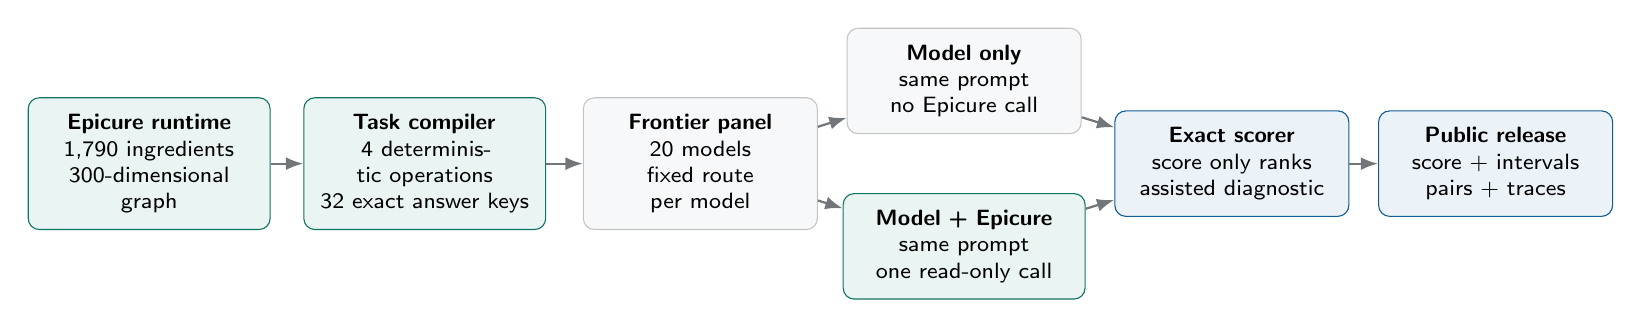
\begin{tikzpicture}[
    x=1cm,y=1cm,font=\sffamily\footnotesize,
    box/.style={draw=FBCharcoal!28,rounded corners=4pt,fill=FBPaper,
      minimum height=1.22cm,text width=2.55cm,align=center,inner sep=6pt},
    oracle/.style={draw=FBTeal!82!black,rounded corners=4pt,fill=FBTeal!9,
      minimum height=1.22cm,text width=2.65cm,align=center,inner sep=6pt},
    score/.style={draw=FBBlue!88!black,rounded corners=4pt,fill=FBBlue!8,
      minimum height=1.22cm,text width=2.55cm,align=center,inner sep=6pt},
    arrow/.style={-{Latex[length=2.2mm]},thick,draw=FBCharcoal!65}
  ]
    \node[oracle] (graph) at (0,0) {\textbf{Epicure runtime}\\1,790 ingredients\\300-dimensional graph};
    \node[oracle] (compiler) at (3.5,0) {\textbf{Task compiler}\\4 deterministic operations\\32 exact answer keys};
    \node[box] (panel) at (7.0,0) {\textbf{Frontier panel}\\20 models\\fixed route per model};
    \node[box] (off) at (10.35,1.05) {\textbf{Model only}\\same prompt\\no Epicure call};
    \node[oracle] (on) at (10.35,-1.05) {\textbf{Model + Epicure}\\same prompt\\one read-only call};
    \node[score] (scorer) at (13.75,0) {\textbf{Exact scorer}\\score only ranks\\assisted diagnostic};
    \node[score] (release) at (17.1,0) {\textbf{Public release}\\score + intervals\\pairs + traces};

    \draw[arrow] (graph) -- (compiler);
    \draw[arrow] (compiler) -- (panel);
    \draw[arrow] (panel) -- (off);
    \draw[arrow] (panel) -- (on);
    \draw[arrow] (off) -- (scorer);
    \draw[arrow] (on) -- (scorer);
    \draw[arrow] (scorer) -- (release);
  \end{tikzpicture}}
  \caption{The \system{} pipeline. \epicure{} fixes each answer before evaluation. The Model only
  arm produces the ranked FlavourBench Score. The matched Model + Epicure arm tests execution with
  the answer-generating system available and does not affect rank. Both reconstruct from the same
  public release.}
  \label{fig:architecture}
\end{figure*}

\section{Epicure reference answers}
\label{sec:oracle}

\subsection{A versioned reference}

For \system{}, ground truth is the output of a specific version of \epicure{}. It is not a claim
about universal culinary preference. The release binds the application, evidence bundle, release
identifier, ingredient count, and embedding dimensionality by hash. A different runtime produces a
different task-set hash.

This definition makes every answer independently recomputable. It also gives the score a direct
interpretation: accuracy is agreement with the published culinary runtime under the published task
construction. No second model decides which response sounds better.

\subsection{Four balanced task families}

The compiler creates eight tasks in each of four families. Seeds and ingredient pairs are fixed
before evaluation. For every task, \epicure{} is called once to obtain the reference result. The
correct answer is extracted programmatically, three distractors are constructed without model
generation, and the four options are shuffled with a task-ID-derived seed.

\begin{table*}[t]
  \centering
  \footnotesize
  \setlength{\tabcolsep}{3pt}
  \begin{tabularx}{\linewidth}{@{}l l X X r@{}}
    \toprule
    Family & Epicure operation & Exact target & Example query & Tasks \\
    \midrule
    Substitution & \texttt{neighbors} & first ranked neighbour & top neighbour for tomato & 8 \\
    Composition & \texttt{pairing\_score} & four-decimal affinity & tomato + basil & 8 \\
    Cookability & \texttt{compare\_on\_axis} & larger flavour projection & coffee vs. chocolate on bitter & 8 \\
    Evidence & \texttt{cultural\_profile} & highest cuisine cosine & cuisine direction for kimchi & 8 \\
    \bottomrule
  \end{tabularx}
  \caption{The task set is balanced by construction. Each family maps one deterministic \epicure{}
  operation to a four-choice answer. Chance accuracy is 25\%.}
  \label{tab:tasks}
\end{table*}

The task families deliberately mix retrieval and computation. Neighbour and cuisine questions test
whether a model knows relationships encoded by the graph. Pairing questions require an exact
numeric result that is difficult to guess. Axis questions test a comparative claim rather than a
memorised scalar. Together they prevent the leaderboard from reducing to one operation or one
kind of culinary trivia.

\subsection{Prompt and answer contract}

Each prompt names the relevant operation and gives four choices. Models may explain briefly, but
the last answer line must be \texttt{FINAL\_CHOICE: X}. The parser accepts A, B, C, or D on that
marker line. A missing marker, abnormal provider finish, timeout, or absent response scores zero.
The rule fits in the standalone verifier shipped with the release.

The complete task set contains no hidden human label and no model-authored item. The benchmark is
therefore suitable for automatic reruns, CI-style regression tests, and training loops where
thousands of candidate responses must be scored consistently.

\section{Evaluation design}
\label{sec:design}

\subsection{One score and one matched intervention}

For model $m$ and task $t$, let $M_{mt}$ equal one when the Model only response finishes normally
and matches the \epicure{} answer. Let $E_{mt}$ be the same indicator for Model + Epicure. The
prompt, route, temperature, top-$p$, seed request, output limit, and answer parser are identical.
Only access to \epicure{} changes.

Each Model + Epicure response may make one read-only call to the operation named in the prompt. The
runner records the operation, arguments, latency, error flag, and a hash of the returned payload.
The returned data is bounded before it enters model context. Automatic provider fallback is
disabled, so a route failure remains a failure for that route.

The single ranking metric is the FlavourBench Score:
\begin{equation}
 F_m = 100\,\frac{1}{32}\sum_t M_{mt}.
 \label{eq:score}
\end{equation}
Every family contains eight tasks, so ordinary accuracy already gives each family equal weight.
Missing or invalid responses remain in the denominator as incorrect. The paper and public Space
give equal values of $F_m$ the same score rank; model name orders rows within a tie. No assisted
metric breaks a FlavourBench Score tie.

Epicure Gain is the matched difference
\begin{equation}
 G_m = 100\,\frac{1}{32}\sum_t\left(E_{mt}-M_{mt}\right),
 \label{eq:uplift}
\end{equation}
reported in percentage points. $G_m$ is not part of the FlavourBench Score. The release also keeps
the four paired outcomes for every task: both correct, Model only correct, Model + Epicure correct,
or neither correct.

\subsection{Completion and uncertainty}

Completion is the fraction of assigned responses that end normally with a parseable final marker.
The score still counts missing responses as incorrect. Reporting completion beside the score keeps
endpoint failure separate from a wrong culinary answer. A zero score with zero completions is not
evidence of zero model capability. For each 32-task accuracy we report a 95\% Wilson interval as a
descriptive uncertainty indicator. The panel is deliberately balanced rather than randomly drawn
from all culinary questions, so the interval is not a population guarantee.

The benchmark is designed for visible differences, not hundredths of a point. One answer changes
the score by 3.125 points. Exact paired McNemar tests comparing the 20/32 leader with each 19/32
runner-up give $p=\FBTopVsSecondP{}$ and $p=\FBTopVsThirdP{}$. These unadjusted descriptive tests,
the overlapping intervals, family breakdowns, and task matrix all point to the same reading: this
release resolves broad separation, not the order of adjacent leaders.

\subsection{Twenty-model frontier panel}

The panel was fixed before the final calls. It includes three GPT-5.6 tiers rather than treating one
deployment as the entire OpenAI family; three Claude 5 tiers; two Gemini tiers; two DeepSeek V4
routes; both current Cohere Command A routes; and a broad set of current independent and open-weight
families. Kimi K3 runs through Kimi's Anthropic-compatible endpoint. Command A Plus and Command A
Reasoning run through Cohere V2 Chat. Qwen 3.8 Max and GLM 5.2 use explicit OpenRouter routes in the
automated batch \cite{kimi2026k3,kimicode2026providers,cohere2026chat,cohere2026tools,
cohere2026reasoning,openrouter2026generation}. The exact 20-row route table appears in
\Cref{app:routes}.

\section{Results}
\label{sec:results}

\subsection{The FlavourBench Score leaderboard}

\FBTopModel{} leads the fixed panel with \FBTopCorrect{}/32 correct and a FlavourBench Score of
\FBTopScore{} (Wilson 95\% interval \FBTopWilsonLow{}--\FBTopWilsonHigh{}). \Cref{tab:leaderboard}
gives the score-only ranking, correct counts, intervals, and parsed-answer counts. The top three differ by
one answer, their intervals overlap substantially, and the paired tests above do not separate the
leader from either runner-up. Across all 19 leader comparisons, Holm adjustment separates only
\FBLeaderHolmSeparated{} rows, \FBLeaderHolmSeparatedNames{}; two are DNF endpoints. Models with no
parseable model-only answer are marked DNF rather than interpreted as the least capable systems.

\begin{figure*}[t]
  \centering
  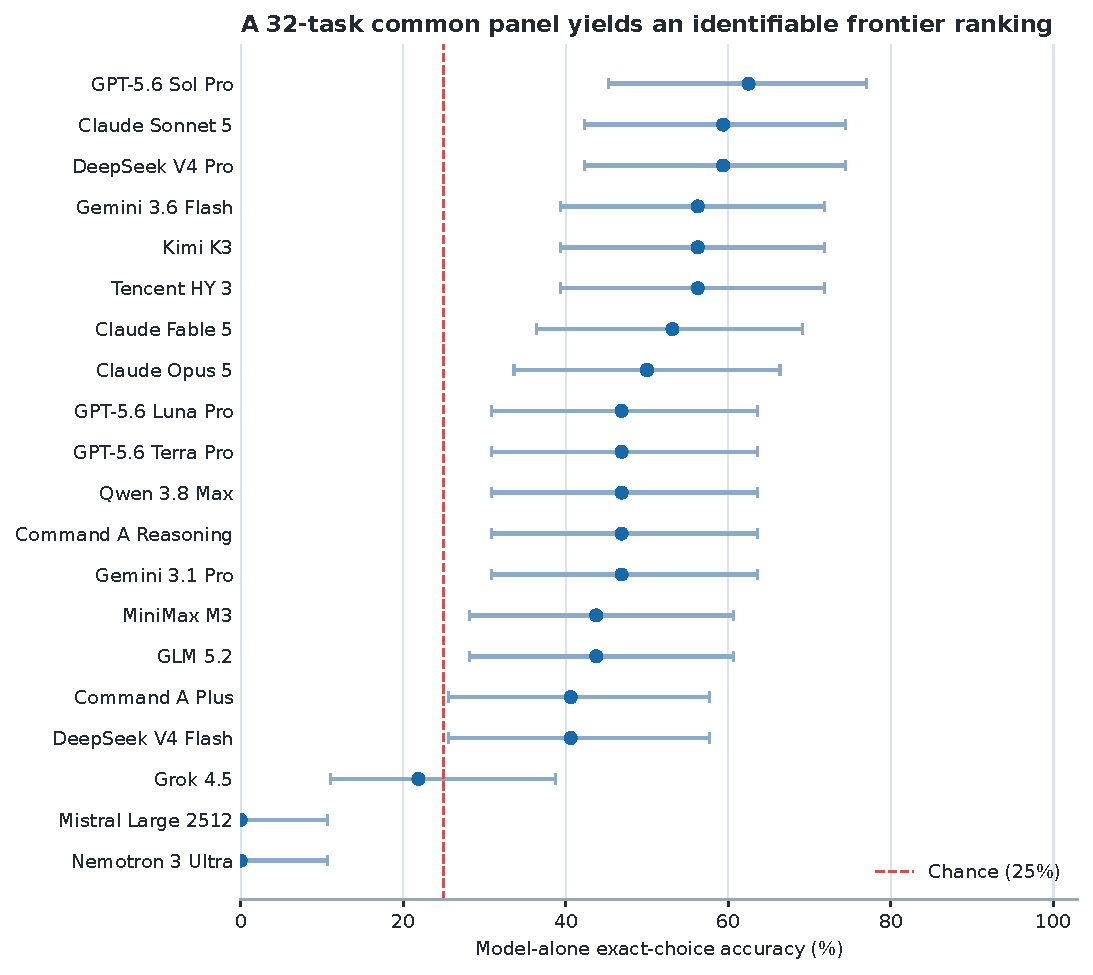
\includegraphics[width=0.88\linewidth]{../figures/epicure-native/frontier-score-forest.pdf}
  \caption{FlavourBench Score against \epicure{} answer keys. Points are exact accuracy over the
  common 32-task panel; bars are descriptive 95\% Wilson intervals. Crosses mark endpoints with no
  parseable model-only answer. The dashed line is four-choice chance.}
  \label{fig:forest}
\end{figure*}

\begin{table*}[t]
  \centering
  \scriptsize
  \setlength{\tabcolsep}{4pt}
  \begin{tabular}{@{}r l r r r r r@{}}
\toprule
Rank & Model & FB Score & +Epicure & Gain & Model \% done & Epicure \% done \\
\midrule
1 & GPT-5.6 Sol Pro & 62.5 & 100.0 & +37.5 & 96.9 & 100.0 \\
2 & Claude Sonnet 5 & 59.4 & 100.0 & +40.6 & 100.0 & 100.0 \\
3 & DeepSeek V4 Pro & 59.4 & 93.8 & +34.4 & 100.0 & 93.8 \\
4 & Gemini 3.6 Flash & 56.2 & 100.0 & +43.8 & 100.0 & 100.0 \\
5 & Kimi K3 & 56.2 & 100.0 & +43.8 & 100.0 & 100.0 \\
6 & Tencent HY 3 & 56.2 & 100.0 & +43.8 & 100.0 & 100.0 \\
7 & Claude Fable 5 & 53.1 & 100.0 & +46.9 & 93.8 & 100.0 \\
8 & Claude Opus 5 & 50.0 & 100.0 & +50.0 & 100.0 & 100.0 \\
9 & GPT-5.6 Luna Pro & 46.9 & 100.0 & +53.1 & 100.0 & 100.0 \\
10 & GPT-5.6 Terra Pro & 46.9 & 100.0 & +53.1 & 100.0 & 100.0 \\
11 & Qwen 3.8 Max & 46.9 & 100.0 & +53.1 & 87.5 & 100.0 \\
12 & Command A Reasoning & 46.9 & 96.9 & +50.0 & 93.8 & 100.0 \\
13 & Gemini 3.1 Pro & 46.9 & 96.9 & +50.0 & 93.8 & 96.9 \\
14 & MiniMax M3 & 43.8 & 100.0 & +56.2 & 96.9 & 100.0 \\
15 & GLM 5.2 & 43.8 & 96.9 & +53.1 & 100.0 & 96.9 \\
16 & Command A Plus & 40.6 & 100.0 & +59.4 & 100.0 & 100.0 \\
17 & DeepSeek V4 Flash & 40.6 & 100.0 & +59.4 & 75.0 & 100.0 \\
18 & Grok 4.5 & 21.9 & 100.0 & +78.1 & 31.2 & 100.0 \\
DNF & Mistral Large 2512 & 0.0 & 93.8 & +93.8 & 0.0 & 100.0 \\
DNF & Nemotron 3 Ultra & 0.0 & 0.0 & +0.0 & 0.0 & 0.0 \\
\bottomrule
\end{tabular}

  \caption{The score-only public leaderboard. ``Correct'' and ``FB Score'' use model-only answers;
  equal scores share a score rank. Wilson 95\% is a descriptive interval for the fixed 32-task
  panel, and ``Parsed'' reports responses with a valid final choice. DNF means that the endpoint
  returned no parseable model-only answer.}
  \label{tab:leaderboard}
\end{table*}

\begin{table*}[t]
  \centering
  \small
  \begin{tabularx}{\linewidth}{@{}>{\raggedright\arraybackslash}p{0.25\linewidth}
      >{\raggedright\arraybackslash}p{0.22\linewidth} X@{}}
    \toprule
    Statistical indicator & Observed value & Reading \\
    \midrule
    Score resolution & 1/32 = 3.125 points & Adjacent rows often differ by one answer. \\
    Leader uncertainty & \FBTopScore\%; Wilson 95\% \FBTopWilsonLow{}--\FBTopWilsonHigh\% &
      Exact for this panel; broad descriptive interval beyond it. \\
    Leader vs. 19/32 runners-up & Exact paired $p=\FBTopVsSecondP{}$ and
      $p=\FBTopVsThirdP{}$ & The fixed panel does not separate the top three. \\
    Leader vs. full panel & \FBLeaderHolmSeparated{}/\FBLeaderHolmComparisons{} comparisons
      significant after Holm adjustment & Only broad operational separation is resolved. \\
    Assisted ceiling & \FBAssistedCeilingModels{}/\FBAssistedEligibleModels{} endpoints at 100\% &
      Useful for integration failures, not rank discrimination. \\
    Score--gain correlation & $r=\FBScoreGainCorrelation{}$ & Near-perfect inverse dependence;
      gain is largely the distance to the assisted ceiling. \\
    \bottomrule
  \end{tabularx}
  \caption{The statistical reading of this release. Intervals and tests are descriptive because
  the 32 tasks form a fixed balanced panel rather than a random sample of all culinary questions.}
  \label{tab:statistical-reading}
\end{table*}

The answer key exists before the model call, every endpoint receives the same questions, and no
judge is sampled after the fact. Missing outputs count as incorrect in the operational score but
remain visible in the ``Parsed'' column. Mistral Large 2512 returned 32 normal model-only
responses, but none contained a parseable final choice. Nemotron 3 Ultra returned no response in
either condition. Both zeroes are operational outcomes rather than capability estimates.

\subsection{What Epicure changes}

The assisted condition is deliberately secondary. Among the \FBAssistedEligibleModels{} endpoints
that returned assisted completions, \FBAssistedCeilingModels{} score 100\% and mean accuracy is
\FBAssistedEligibleAccuracy\%. FlavourBench Score and Epicure Gain correlate
$r=\FBScoreGainCorrelation{}$ because a near-100\% assisted ceiling makes gain approximately
$100-F_m$. Gain therefore adds little ranking information and does not appear in the primary table.

\begin{figure*}[t]
  \centering
  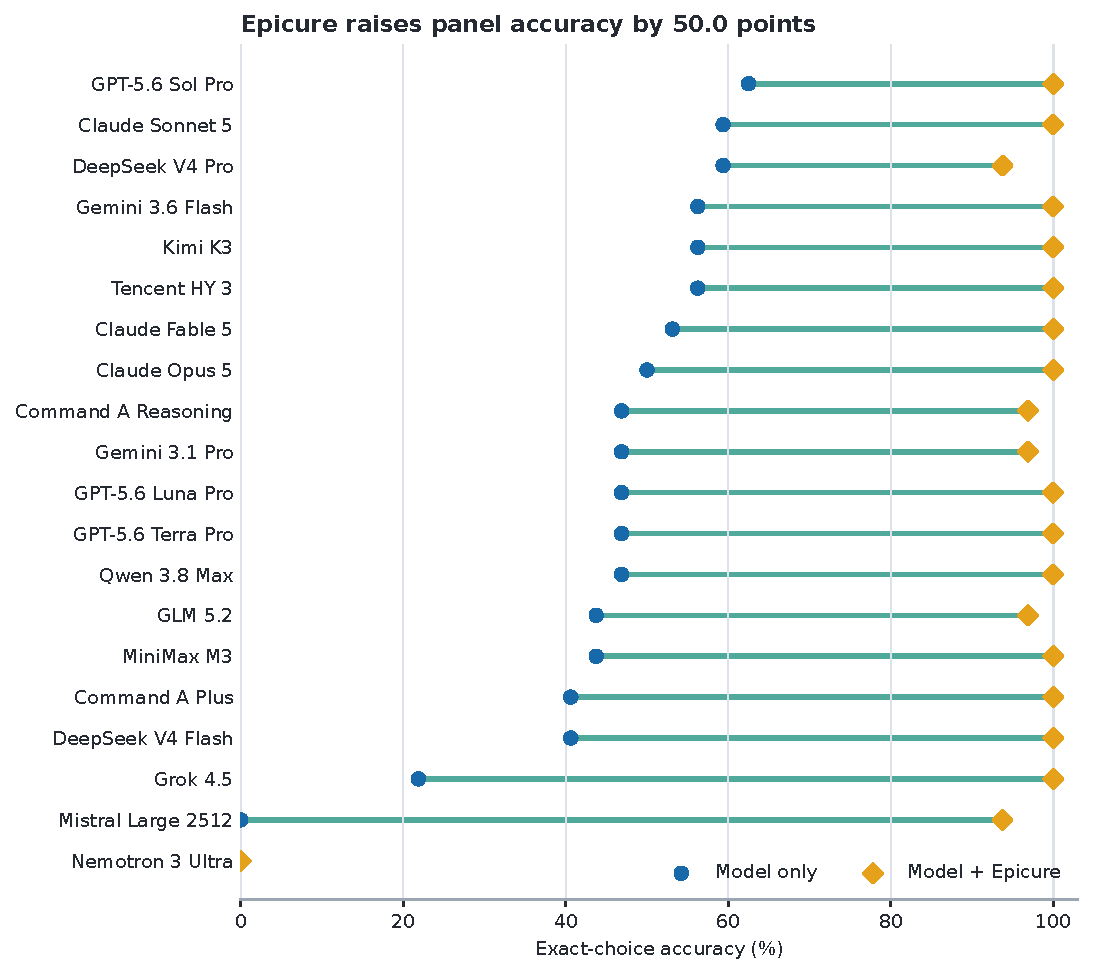
\includegraphics[width=0.88\linewidth]{../figures/epicure-native/frontier-score-dumbbell.pdf}
  \caption{Model-only and named-operation assisted accuracy over the same 32 tasks. This secondary
  diagnostic shows the assisted ceiling and endpoint failures; it does not determine rank.}
  \label{fig:dumbbell}
\end{figure*}

The assisted prompt names the relevant operation, whose output is also used to compile the answer
key. Near-ceiling assisted accuracy is therefore expected. The condition tests whether an endpoint
can call the specified operation, read its output, and preserve the answer contract. It is not an
independent validation of \epicure{}, a second capability score, or a test of open-ended tool
discovery.

\subsection{Families explain aggregate ties}

The four task families have different demands. Pairing questions require an exact four-decimal
value; substitution and cultural questions can sometimes be answered from broad food knowledge;
axis comparisons require a directional decision in \epicure{}'s latent space. \Cref{fig:heatmap}
shows that similar total scores can arise from different profiles.



\begin{table}[t]
  \centering
  \scriptsize
  \resizebox{\columnwidth}{!}{%
    \begin{tabular}{@{}l l r r r@{}}
\toprule
Family & Epicure operation & Tasks & Model only & Model + Epicure \\
\midrule
Substitution & \texttt{neighbors} & 8 & 18.1 & 94.4 \\
Composition & \texttt{pairing\_score} & 8 & 40.6 & 94.4 \\
Cookability & \texttt{compare\_on\_axis} & 8 & 62.5 & 92.5 \\
Evidence & \texttt{cultural\_profile} & 8 & 54.4 & 94.4 \\
\bottomrule
\end{tabular}
%
  }
  \caption{Panel-average performance by family and the corresponding reference operation.}
  \label{tab:families}
\end{table}

\subsection{Every model and task pair is inspectable}

Aggregate bars can hide a benchmark bug or a single pathological task. \Cref{fig:matrix} therefore
publishes all 640 paired outcomes. Blue cells are stable knowledge: both conditions are correct.
Gold cells are Epicure wins: Model only is wrong and Model + Epicure is correct. Red cells show the
reverse outcome. Grey cells show questions neither condition solved.



\subsection{Cohere, Kimi, Qwen, and route fidelity}

Both Cohere models are full members of the public panel. Command A Plus has score rank
\FBCoherePlusRank{} with a FlavourBench Score of \FBCoherePlusScore{}; Command A Reasoning has
score rank \FBCohereReasoningRank{} at \FBCohereReasoningScore{}. Kimi K3 has score rank
\FBKimiRank{} through the direct Kimi endpoint. Qwen 3.8 Max has score rank \FBQwenRank{} through
an exact OpenRouter route, and GLM 5.2 has score rank \FBGLMRank{}. No route changes during
generation.

The two direct Cohere routes each produced all 64 assigned arms. Their returned identifiers are
\texttt{\seqsplit{command-a-plus-05-2026}} and
\texttt{\seqsplit{command-a-reasoning-08-2025}}, respectively; the direct Kimi route likewise
produced all 64 arms under returned identifier \texttt{k3}. The offline verifier checks these
provider, identity, and arm-count contracts before accepting the release.

This matters because a model name is not a transport contract. The release stores the requested
model, returned model, provider, route, generation ID, latency, token counts, and response hash.
Direct and routed endpoints can therefore be analysed separately without pretending they are
interchangeable deployments.

\subsection{Score and response time}

\Cref{fig:latency} plots FlavourBench Score against median response time. Marker colour identifies
the execution route. Accuracy and latency are separate operational dimensions: faster endpoints do
not necessarily score higher, and direct-provider routes are not pooled with routed deployments.



\section{Using the score as a training signal}
\label{sec:training}

The same environment exposes four binary indicators for a generated trajectory $\tau$:
$r_{\mathrm{answer}}$ for a correct answer, $r_{\mathrm{format}}$ for a parseable final marker,
$r_{\mathrm{call}}$ for a successful Epicure call, and $r_{\mathrm{align}}$ for a call matching the
reference operation. The public leaderboard uses $r_{\mathrm{answer}}$ in Model only. A future
training objective could use
\begin{equation}
 r(\tau)=r_{\mathrm{answer}}r_{\mathrm{format}}
 +\lambda r_{\mathrm{answer}}r_{\mathrm{call}}
 +\mu r_{\mathrm{align}},
 \label{eq:reward}
\end{equation}
where each component is a binary indicator and $\lambda,\mu$ set the value of successful and
reference-matching calls. Requiring a correct answer prevents irrelevant calls from earning the
main reward. The interface could support rejection sampling, preference optimisation, or
reinforcement learning on new ingredient seeds. This paper does not train a checkpoint; such a
study should keep the public leaderboard as a final evaluation split.

\section{Reproducibility and release}
\label{sec:reproduction}

The public release is one JSON document with hash \FBReleaseSHA{}. It contains the 20 route records,
32 full prompts, answer keys and reference \epicure{} results, 1,280 observation rows, final answer
markers, response times, and bounded Epicure-trace projections. \FBObservedArms{} provider responses
were observed; \FBMissingArms{} missing arms remain explicit zero-scored rows.

The leaderboard can be reconstructed without a network connection, provider key, GPU, or running
\epicure{} service:

\begin{verbatim}
python3 -I reproduce_epicure_native.py \
  --release generated/epicure-native/\
  epicure-native-release.json
\end{verbatim}

The verifier rejects duplicate JSON keys, non-finite numbers, a changed content address, an
incomplete $20\times32\times2$ grid, or any leaderboard value that differs from recomputation. The
paper tables and figures are generated from the same release, so a changed score cannot leave a
stale chart behind.

Reproducing the original hosted calls is a different operation from replaying the result. The
release records exact routes and request policies, but provider deployments can change. A fresh
frontier run should generate a new manifest and release rather than overwrite this snapshot.

\section{Discussion}
\label{sec:discussion}

\paragraph{What the score means.}
The FlavourBench Score answers a narrow operational question: how often did this deployed endpoint
return the answer fixed by the published \epicure{} runtime? It includes endpoint availability
because missing responses score zero. The completion columns reveal that component. The score is
not a universal measure of cooking skill, but it is exact, reproducible, and independent of a
model judge.

\paragraph{Do we need humans?}
Not for this leaderboard. Humans are useful when the target is preference, creativity, safety, or
the quality of an open-ended recipe. They are unnecessary when the question is whether a model's
choice matches a deterministic runtime result. \system{} uses that distinction to automate the
core ranking while leaving subjective culinary evaluation as a separate track.

\paragraph{Why run Model + Epicure?}
The condition is a named-operation execution test. Because \epicure{} both generated the answer
key and supplies the relevant runtime output, its near-ceiling accuracy is expected. The condition
still catches tool-call, argument, parsing, and answer-contract failures, but it neither ranks
models nor independently validates \epicure{}. The dumbbell and pair matrix expose those failures
task by task.

\paragraph{Scaling the benchmark.}
The task compiler can expand the seed lists while preserving the four operations. The next release
should reserve unseen ingredients and pairs, remove near-duplicate questions, and measure stability
across runtime versions. As a simple scale guide near 50\% accuracy, 100 independent tasks give
about a 10-point 95\% half-width and 400 give about five points; paired rank claims should be powered
on the observed task covariance. The current panel is a frontier snapshot and a reproducible
template for that larger hidden set.

\section{Related work}

HELM argues for explicit scenarios and metrics, while recent benchmark audits emphasise validity,
contamination, and transparent reporting \cite{liang2022helm,reuel2024betterbench}. Chatbot Arena
and WildBench evaluate broad answer quality through preferences or checklists
\cite{chiang2024chatbotarena,lin2024wildbench}. \system{} instead targets an executable domain model
and needs no judge for its primary score.

ToolLLM, BFCL, and $\tau$-bench make tool invocation or environment state observable
\cite{qin2023toolllm,patil2025bfcl,yao2024taubench}. \system{} adds a matched Model only condition,
so \epicure{} becomes an intervention rather than a requirement shared by every response. LiveBench,
LiveCodeBench, GPQA, MMLU-Pro, and SWE-bench illustrate complementary strategies for reducing
contamination or grounding answers in difficult tasks and executable outcomes
\cite{white2024livebench,jain2024livecodebench,rein2023gpqa,wang2024mmlupro,jimenez2023swebench}.

\begin{table*}[t]
  \centering
  \small
  \begin{tabularx}{\linewidth}{@{}>{\raggedright\arraybackslash}p{0.19\linewidth}
      >{\raggedright\arraybackslash}p{0.20\linewidth} X c@{}}
    \toprule
    Benchmark & Scope & Primary target & \shortstack{Paired\\tool?} \\
    \midrule
    Chatbot Arena & general chat & pairwise human preference & No \\
    WildBench & general chat & task-specific checklist & No \\
    BFCL & function calling & executable call match & No \\
    $\tau$-bench & interactive agents & exact goal state & No \\
    DiningBench & multimodal food & dish and nutrition labels & No \\
    FAM-Bench & food-as-medicine & expert suitability label & No \\
    \system{} & culinary reasoning & versioned executable \epicure{} operation & Yes \\
    \bottomrule
  \end{tabularx}
  \caption{\system{} complements broad, tool-use, and food-domain benchmarks. Its distinctive unit
  is the same endpoint and task measured as Model only and Model + Epicure; ``paired tool'' denotes
  that matched intervention rather than ordinary tool availability.}
  \label{tab:benchmark-comparison}
\end{table*}

Culinary datasets such as FlavorDB and Recipe1M organise ingredient and recipe evidence
\cite{garg2018flavordb,salvador2017recipe1m}. Recent food benchmarks emphasise other constructs:
NutriBench estimates carbohydrates from meal descriptions; FoodBench-QA grounds nutrition tasks in
databases and ontologies; DiningBench tests multimodal dish perception and nutrition reasoning; and
FAM-Bench evaluates condition-aware food-as-medicine decisions
\cite{hua2025nutribench,eftimov2026foodbench,jin2026diningbench,mao2026fambench}. CookingSense and
planning-oriented culinary work test commonsense and procedures
\cite{choi2024cookingsense,wu2025recipe2plan}. \system{} targets a complementary construct:
ingredient-space flavour decisions whose targets are compiled from a callable, versioned runtime,
with access to that runtime measured as a matched intervention.

\section{Limitations}

The 32-task panel resolves broad differences, not adjacent leaders: one answer moves the score by
3.125 points and the leading intervals overlap. The English ingredient seeds cover four
\epicure{} operations, hosted routes are a dated snapshot, and public prompts may eventually be
memorised. Agreement with \epicure{} inherits the runtime's representation choices; it is not a
food-safety or cultural-authenticity certification. A larger hidden panel, additional operations,
and repeated route snapshots are the immediate next tests.

\section{Conclusion}

\system{} turns a versioned culinary runtime into an executable benchmark for frontier language
models. \FBTopModel{} leads this 20-model, 32-task snapshot at \FBTopScore{}\%, while the overlapping
leading intervals make the close group explicit. Scores, completions, prompts, responses, and
traces all reconstruct from the released 1,280-arm grid. The result is a simple automated
leaderboard with a separate named-operation diagnostic, not a model judge hidden behind another
score.

\clearpage
\appendix

\section{Real prompts, answers, and tool calls}
\label{sec:cases}

A benchmark paper should show what was actually asked. The four cases below are selected
mechanically, one per family. Where possible, the builder chooses a model and task that is wrong in
Model only and correct in Model + Epicure. Each case includes the full prompt, both final answers,
the actual operation and arguments, and the exact answer key.

\paragraph{Case 1: Substitution with GPT-5.6 Sol Pro.}
\textbf{Prompt.} FlavourBench Epicure-native exact task. Use the read-only culinary evidence tools if they are available; otherwise answer from your own knowledge.

According to Epicure's `neighbors` result for `tomato` with top\_k=4, which ingredient is ranked first?

Choices:
A. oregano
B. bell\_pepper
C. olive\_oil
D. onion

In your final answer, explain briefly if useful and finish on its own line with exactly `FINAL\_CHOICE: X`, replacing X with A, B, C, or D.

\textbf{Model alone.} \texttt{FINAL\_CHOICE: D} \quad \textbf{With Epicure.} \texttt{FINAL\_CHOICE: B}

\textbf{Epicure call.} \texttt{neighbors}\allowbreak\texttt{(\{"ingredient": "tomato", "top\_k": 4\})}. The answer key is \texttt{FINAL\_CHOICE: B}.

\textbf{Epicure result.} {\ttfamily\footnotesize\sloppy \{"ingredient": "tomato", "neighbors": [\{"name": "bell\_pepper", "rank": 1, "sim": 0.4799\}, \{"name": "olive\_oil", "rank": 2, "sim": 0.4786\}, \{"name": "oregano", "rank": 3, "sim": 0.4646\}, \{"name": "onion", "rank": 4, "sim": 0.4567\}]\}}

\paragraph{Case 2: Composition with DeepSeek V4 Pro.}
\textbf{Prompt.} FlavourBench Epicure-native exact task. Use the read-only culinary evidence tools if they are available; otherwise answer from your own knowledge.

What exact four-decimal `pairing\_score` does Epicure return for `tomato` and `basil`?

Choices:
A. 0.2707
B. 0.2407
C. 0.3207
D. 0.1907

In your final answer, explain briefly if useful and finish on its own line with exactly `FINAL\_CHOICE: X`, replacing X with A, B, C, or D.

\textbf{Model alone.} \texttt{FINAL\_CHOICE: B} \quad \textbf{With Epicure.} \texttt{FINAL\_CHOICE: A}

\textbf{Epicure call.} \texttt{pairing\_score}\allowbreak\texttt{(\{"ingredient\_a": "tomato", "ingredient\_b": "basil"\})}. The answer key is \texttt{FINAL\_CHOICE: A}.

\textbf{Epicure result.} {\ttfamily\footnotesize\sloppy \{"all\_pairs\_range": \{"median": 0.092, "p10": 0.0197, "p25": 0.0521, "p75": 0.1392, "p90": 0.1899\}, "pairing\_score": 0.2707, "percentile\_label": "very high (>=p90)", "resolved\_a": "tomato", "resolved\_b": "basil"\}}

\paragraph{Case 3: Cookability with GPT-5.6 Sol Pro.}
\textbf{Prompt.} FlavourBench Epicure-native exact task. Use the read-only culinary evidence tools if they are available; otherwise answer from your own knowledge.

Which statement matches Epicure's `compare\_on\_axis` result for `coffee` versus `chocolate` on `cf\_bitter`?

Choices:
A. coffee has the higher projection
B. the projections are equal to four decimals
C. Epicure cannot resolve one or both ingredients
D. chocolate has the higher projection

In your final answer, explain briefly if useful and finish on its own line with exactly `FINAL\_CHOICE: X`, replacing X with A, B, C, or D.

\textbf{Model alone.} \texttt{FINAL\_CHOICE: A} \quad \textbf{With Epicure.} \texttt{FINAL\_CHOICE: D}

\textbf{Epicure call.} \texttt{compare\_on\_axis}\allowbreak\texttt{(\{"axis": "cf\_bitter", "ingredient\_a": "coffee", "ingredient\_b": "chocolate"\})}. The answer key is \texttt{FINAL\_CHOICE: D}.

\textbf{Epicure result.} {\ttfamily\footnotesize\sloppy \{"axis": "cf\_bitter", "axis\_range": \{"p10": -0.0877, "p90": 0.1429\}, "delta": 0.0835, "label\_a": "moderate", "label\_b": "high", "projection\_a": 0.0076, "projection\_b": 0.0911, "resolved\_a": "coffee", "resolved\_b": "chocolate"\}}

\paragraph{Case 4: Evidence with Grok 4.5.}
\textbf{Prompt.} FlavourBench Epicure-native exact task. Use the read-only culinary evidence tools if they are available; otherwise answer from your own knowledge.

Which cuisine direction has the highest cosine score in Epicure's `cultural\_profile` result for `miso`?

Choices:
A. Japanese
B. East\_Asian
C. Southeast\_Asian
D. South\_Asian

In your final answer, explain briefly if useful and finish on its own line with exactly `FINAL\_CHOICE: X`, replacing X with A, B, C, or D.

\textbf{Model alone.} \texttt{\{"name": "cultural\_profile", "arguments": \{"ingredient": "miso"\}\}} \quad \textbf{With Epicure.} \texttt{FINAL\_CHOICE: A}

\textbf{Epicure call.} \texttt{cultural\_profile}\allowbreak\texttt{(\{"ingredient": "miso"\})}. The answer key is \texttt{FINAL\_CHOICE: A}.

\textbf{Epicure result.} {\ttfamily\footnotesize\sloppy \{"cuisines": \{"East\_Asian": \{"range": \{"p10": -0.1649, "p90": 0.3039\}, "score": 0.1625\}, "Eastern\_European": \{"range": \{"p10": -0.1466, "p90": 0.1034\}, "score": -0.1494\}, "Japanese": \{"range": \{"p10": -0.1359, "p90": 0.1896\}, "score": 0.3227\}, "Latin\_American": \{"range": \{"p10": -0.1672, "p90": 0.1281\}, "score": -0.1538\}, "Mediterranean": \{"range": \{"p10": -0.2323, "p90": 0.206\}, "score": -0.1198\}, "South\_Asian": \{"range": \{"p10": -0.0808, "p90": 0.071\}, "score": -0.0585\}, "Southeast\_Asian": \{"range": \{"p10": -0.1625, "p90": 0.193\}, "score": 0.0426\}, "Western\_Atlantic": \{"range": \{"p10": -0.2304, "p90": 0.183\}, "score": -0.1546\}\}, "note": "Cosine similarity to each cuisine direction. Use p10/p90 to judge whether a score is typical or extreme.", "resolved": "miso"\}}


These examples show exactly what the two measurements contain. Model only tests knowledge or
inference about the hidden graph. Model + Epicure names the operation, so it tests whether the
model can form valid arguments, read the returned structure, and preserve the answer contract. A
correct choice with the wrong operation still earns answer credit, but the release separately
reports whether the reference operation was matched. Across the run there are \FBToolCalls{}
projected \epicure{} calls and \FBReferenceMatches{} model and task pairs matching the reference
operation.

\section{Additional result figures}

\begin{figure*}[t]
  \centering
  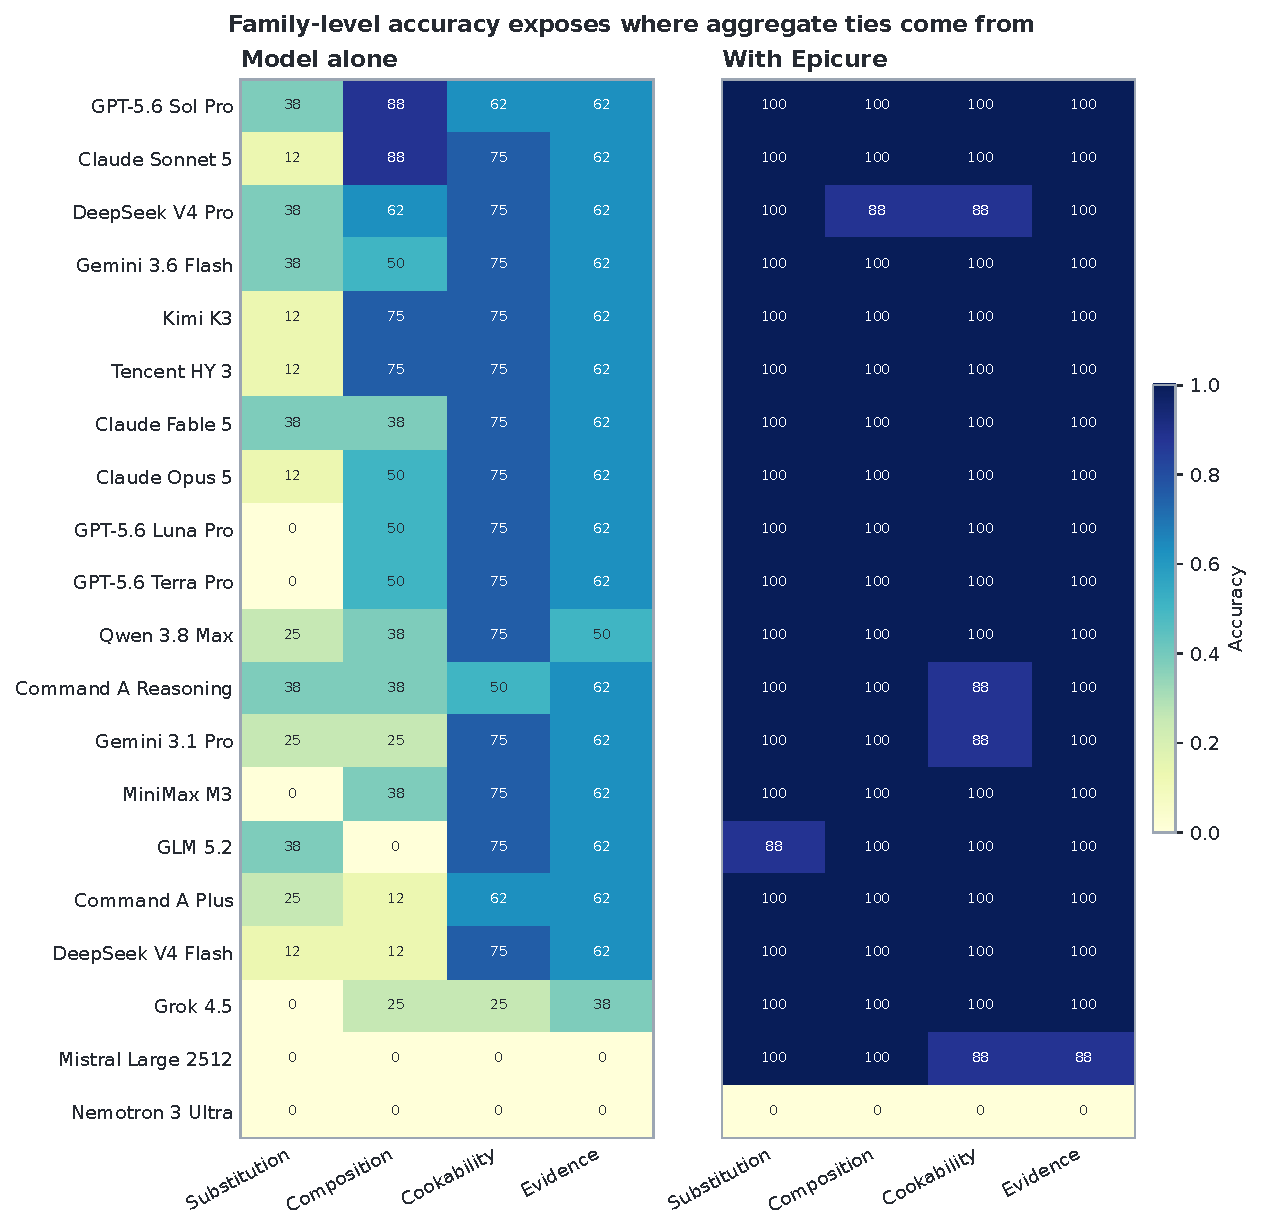
\includegraphics[width=0.95\linewidth]{../figures/epicure-native/frontier-family-heatmap.pdf}
  \caption{Model only and Model + Epicure accuracy by task family. Each value is a percentage over
  eight tasks. Similar FlavourBench Scores can come from different family profiles.}
  \label{fig:heatmap}
\end{figure*}

\begin{figure*}[t]
  \centering
  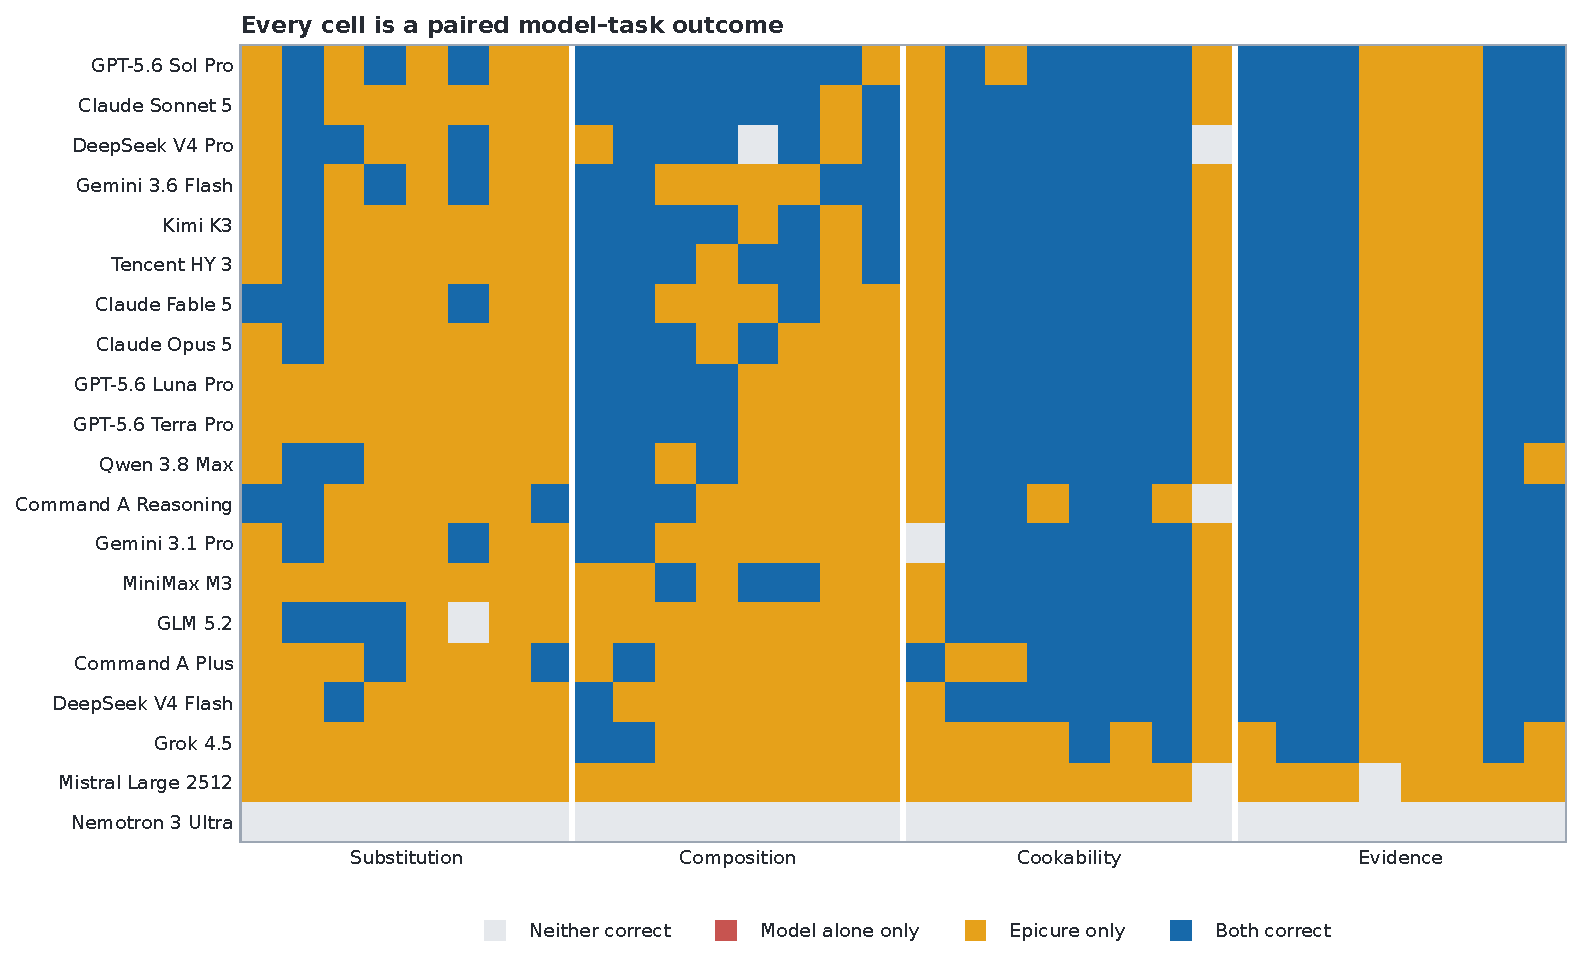
\includegraphics[width=\linewidth]{../figures/epicure-native/frontier-paired-outcome-matrix.pdf}
  \caption{All 640 matched outcomes, ordered by FlavourBench Score and grouped by task family. The
  matrix shows which exact tasks produce Epicure Gain and where the assisted response regresses.}
  \label{fig:matrix}
\end{figure*}

\begin{figure*}[t]
  \centering
  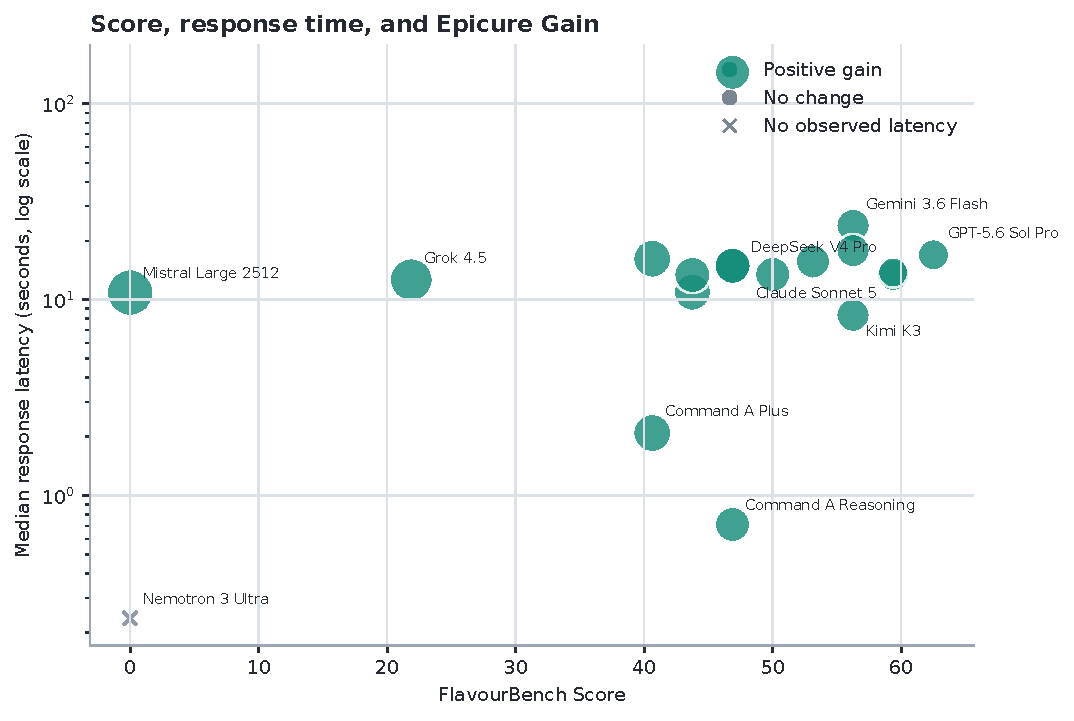
\includegraphics[width=0.82\linewidth]{../figures/epicure-native/frontier-latency-uplift.pdf}
  \caption{FlavourBench Score and response time. Response time uses a log scale; colour identifies
  direct-provider and OpenRouter execution. An $\times$ marks a route with no observed response
  time.}
  \label{fig:latency}
\end{figure*}

\section{Exact execution routes}
\label{app:routes}

\begin{table}[h!]
  \centering
  \resizebox{\columnwidth}{!}{%
    \begin{tabular}{@{}r l l@{}}
\toprule
Slot & Model & Execution route \\
\midrule
1 & GPT-5.6 Sol Pro & openrouter: openai/flex \\
6 & Claude Sonnet 5 & openrouter: amazon-bedrock/claude-on-aws \\
13 & DeepSeek V4 Pro & openrouter: baidu/fp8 \\
8 & Gemini 3.6 Flash & openrouter: google-vertex/global/flex \\
10 & Kimi K3 & kimi\_direct: kimi-code-direct \\
18 & Tencent HY 3 & openrouter: baidu/fp8 \\
4 & Claude Fable 5 & openrouter: amazon-bedrock \\
5 & Claude Opus 5 & openrouter: amazon-bedrock/claude-on-aws \\
3 & GPT-5.6 Luna Pro & openrouter: openai/flex \\
2 & GPT-5.6 Terra Pro & openrouter: openai/flex \\
11 & Qwen 3.8 Max & openrouter: alibaba \\
20 & Command A Reasoning & cohere\_direct: cohere-direct \\
7 & Gemini 3.1 Pro & openrouter: google-vertex/global/flex \\
15 & MiniMax M3 & openrouter: together \\
12 & GLM 5.2 & openrouter: coreweave/fp4 \\
19 & Command A Plus & cohere\_direct: cohere-direct \\
14 & DeepSeek V4 Flash & openrouter: cloudflare/fp8 \\
9 & Grok 4.5 & openrouter: xai/zdr \\
17 & Mistral Large 2512 & openrouter: mistral \\
16 & Nemotron 3 Ultra & openrouter: deepinfra/fp4 \\
\bottomrule
\end{tabular}
%
  }
  \caption{All 20 model routes in the released leaderboard. Routes are selected before generation;
  automatic fallback is disabled.}
  \label{tab:routes}
\end{table}

\section{Protocol details}

All arms request temperature 0, top-$p$ 1, and seed 20260810 where the provider supports it. The
final response budget is 2,048 tokens. Model + Epicure has one call round, one call total, a
4,096-byte result bound, and a 4,096-byte cumulative result bound. At most two provider attempts
are allowed, and an ambiguously delivered request is never replayed. The final marker is parsed
from plain text for transport portability; direct providers may use native structured generation
internally and normalize to the same marker.

\section{Data fields}

Each observation binds model ID, task ID, condition, source status, source and response hashes,
returned model and provider, finish reason, response time, final answer, observed and expected
choice, normal-parse flag, correctness, and a projected Epicure trace. Each trace event contains its
name, structured arguments, error flag, response time, and result hash. The release does not require
raw provider credentials or hidden service state.

% Flush benchmark figures and appendix tables before the references so the
% empirical story remains contiguous in the compiled paper.

\clearpage
\label{references-start}
{\small
\bibliographystyle{plainnat}
\bibliography{references}
}

\clearpage
\input{checklist-answers.tex}

\end{document}
